\chapter{Mô hình phân loại điện tâm đồ }
\thispagestyle{fancy}

\section{Sơ lược về bộ dữ liệu sử dụng trong nghiên cứu}
\subsection{Giới thiệu}
Bộ dữ liệu Loạn nhịp tim MIT-BIH (MIT-BIH Arrhythmia Database) là một trong những bộ dữ liệu về điện tim nổi tiếng nhất, được sử dụng phổ biến ở rất nhiều các nghiên cứu về điện tim trên toàn thế giới. Bộ dữ liệu được thu thập từ những trung tâm y tế, nghiên cứu hàng đầu qua nhiều công đoạn xử lý tín hiệu và được xem xét bởi những y bác sĩ uy tín. Bộ dữ liệu thể hiện rõ những bất thường tim mạch cũng như có những ghi chú chi tiết trên từng bệnh nhân đem lại cho nhưng nghiên cứu khoa học một nguồn tư liệu dồi dào và chính xác.
\subsection{Nguồn thu thập dữ liệu}
Physionet à một trang web truy cập miễn phí các bộ dữ liệu lớn về tín hiệu sinh lý được ghi lại (PhysioBank) và những phần mềm mã nguồn mở liên quan (PhysioToolkit).
\begin{center}
    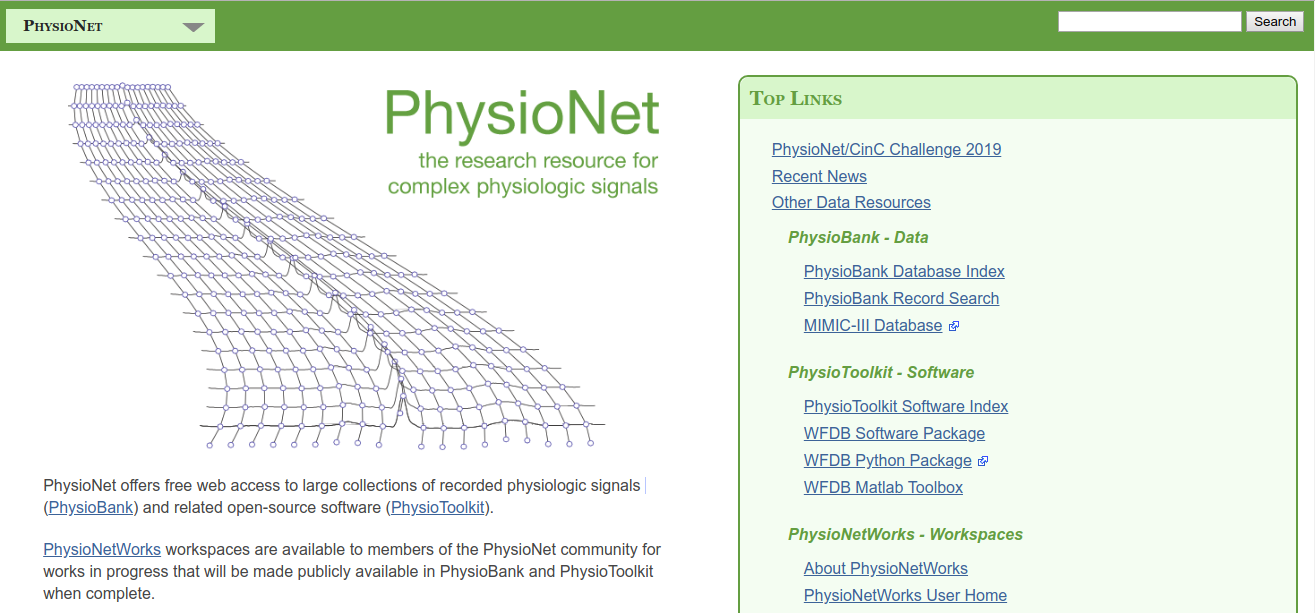
\includegraphics[scale=.3]{image/chapter2/Screenshot_from_2019-03-11_04-58-18.png}
    \begin{figure}[htp]
    \begin{center}
    \end{center}
    \caption{Trang Physionet}
    \end{figure}
\end{center}

\subsection{Thông tin về database}
Từ năm 1975, các phòng thí nghiệm tại Bệnh viện Beth Israel của Boston (nay là Trung tâm Y tế Beth Israel Deaconess) và tại MIT đã hỗ trợ nghiên cứu về phân tích rối loạn nhịp tim và các đối tượng liên quan. Một trong những sản phẩm chính đầu tiên của nỗ lực đó là Cơ sở dữ liệu Chứng loạn nhịp tim MIT-BIH, chúng tôi đã hoàn thành và bắt đầu phân phối vào năm 1980.\cite{mitbih}
Cơ sở dữ liệu Chứng loạn nhịp tim MIT-BIH chứa 48 trích đoạn nửa tiếng của các bản ghi ECG lưu động hai kênh, thu được từ 47 đối tượng được nghiên cứu bởi Phòng thí nghiệm Chứng loạn nhịp tim BIH từ năm 1975 đến 1979. Đối tượng là 25 nam từ 32 đến 89 tuổi và 22 nữ từ 23 đến 89 tuổi. Hai mươi ba bản ghi được chọn ngẫu nhiên từ bộ 4000 dữ liệu 24 tiếng Các bản ghi ECG lưu động  được thu thập từ một nhóm bệnh nhân nội trú hỗn hợp (khoảng 60\%) và bệnh nhân ngoại trú (khoảng 40\%) tại Bệnh viện Beth Israel của Boston; 25 bản ghi còn lại được chọn từ cùng một bộ để bao gồm các rối loạn nhịp tim ít phổ biến hơn nhưng có ý nghĩa lâm sàng sẽ không được thể hiện tốt trong một mẫu ngẫu nhiên nhỏ.
Nhóm đầu tiên được dự định là một mẫu đại diện cho sự đa dạng của dạng sóng và nhiễu mà một máy phát hiện rối loạn nhịp tim có thể gặp phải trong sử dụng lâm sàng thông thường. Các hồ sơ trong nhóm thứ hai đã được chọn để bao gồm rối loạn nhịp thất, rối loạn chức năng và thất trái phức tạp và bất thường dẫn truyền. Một vài trong số các hồ sơ này đã được chọn vì các đặc điểm của nhịp điệu, biến thể hình thái QRS hoặc chất lượng tín hiệu có thể được dự kiến sẽ gây khó khăn đáng kể cho các máy phát hiện rối loạn nhịp tim; những hồ sơ này đã đạt được sự nổi tiếng đáng kể trong số những người sử dụng cơ sở dữ liệu.

Các bản ghi được số hóa ở 360 mẫu mỗi giây trên mỗi kênh với độ phân giải 11-bit trên phạm vi 10 mV. Hai hoặc nhiều bác sĩ tim mạch chú thích độc lập mỗi hồ sơ; những bất đồng đã được giải quyết để có được các chú thích tham chiếu có thể đọc được trên máy tính cho mỗi nhịp (khoảng 110.000 chú thích trong tất cả) kèm theo cơ sở dữ liệu.
% \begin{center}
%     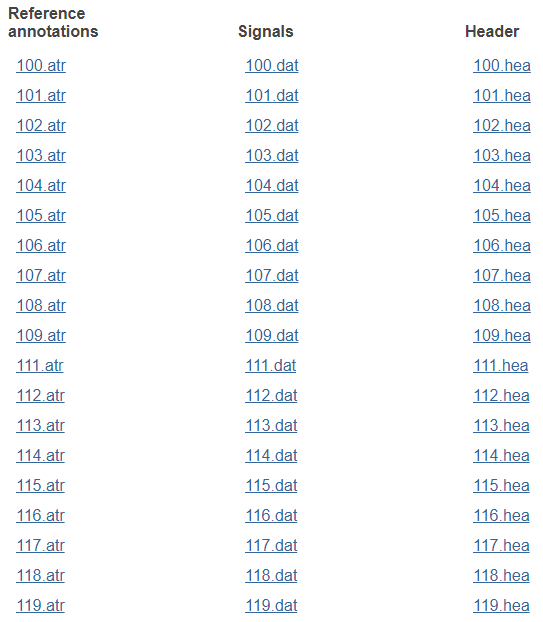
\includegraphics[scale=.4]{image/week3/mit.png}
%     \begin{figure}[htp]
%     \begin{center}
%     \end{center}
%     \caption{Dataset sample}
%     \end{figure}
% \end{center}
\subsubsection{Cấu trúc chuyển đạo và ghi chú}
\begin{center}
    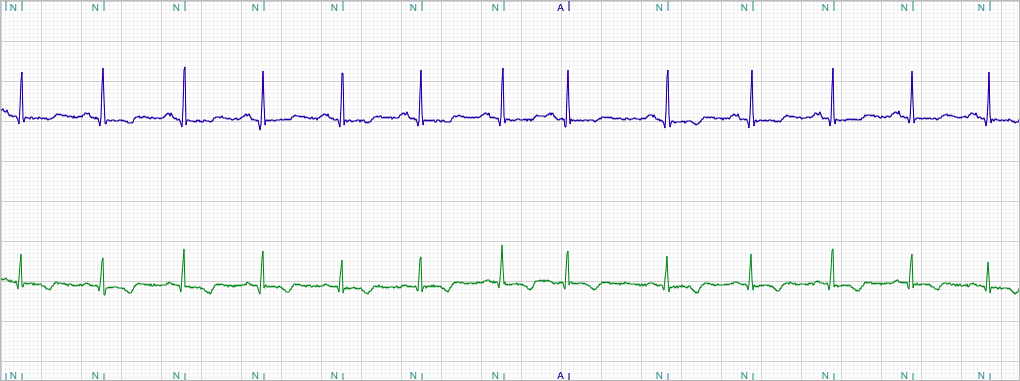
\includegraphics[scale=.4]{image/chapter2/100bee.png}
    \begin{figure}[htp]
    \begin{center}
    \end{center}
    \caption{Ghi chú trên bản ghi thứ 100}
    \end{figure}
\end{center}
Trong hầu hết các bản ghi, tín hiệu trên là modified limb lead II (MLII), thu được bằng cách đặt các điện cực trên ngực. Tín hiệu thấp hơn thường là đạo trình sửa đổi V1 (đôi khi V2 hoặc V5 và trong một trường hợp V4); đối với tín hiệu trên, các điện cực cũng được đặt trên ngực. Cấu hình này được sử dụng thường xuyên bởi Phòng thí nghiệm loạn nhịp tim BIH. Các phức bộ QRS bình thường thường nổi bật trong tín hiệu trên. Tuy nhiên, trục dẫn cho tín hiệu thấp hơn có thể gần trực giao với trục điện tim trung bình, tuy nhiên (tức là, nhịp đập bình thường thường là hai pha và có thể gần như đẳng điện). Do đó, nhịp đập bình thường thường khó phân biệt ở tín hiệu thấp hơn, mặc dù nhịp đập ngoài tử cung thường sẽ nổi bật hơn (xem, ví dụ, ghi 106). Một ngoại lệ đáng chú ý là bản ghi 114, trong đó các tín hiệu bị đảo ngược. Vì điều này thỉnh thoảng xảy ra trong thực hành lâm sàng, máy dò loạn nhịp tim nên được trang bị để đối phó với tình huống này. Trong hồ sơ 102 và 104, không thể sử dụng chì II đã được sửa đổi vì băng phẫu thuật trên bệnh nhân; chì V5 được sửa đổi đã được sử dụng cho tín hiệu trên trong các bản ghi này.

Tại mỗi đỉnh sóng R sẽ được đánh ghi chú cho sóng đó. Ban đầu bộ nhãn đánh dấu trên tập dữ liệu được tạo ra bằng một máy dò phức bộ QRS và đánh dấu nhịp đó là bình thường. Sau đó bộ dữ liệu được đánh nhãn lại. Mỗi bản ghi được đánh nhãn lại một cách chính xác hơn bằng những bác sĩ chuyên khoa tim mạch. Các bác sĩ đã thêm vào các nhãn bổ sung một cách chính xác hơn những nhãn đã đánh, các nhịp bị lỗi cũng như xóa các phát hiện sai lầm.

\subsubsection{Ghi chú trên tập dữ liệu}
\begin{center}
    \begin{tabular}{|c|c|}
         \hline
         Symbol & Meaning \\
         \hline
         . or N & Normal beat \\
         \hline
         L & Left bundle branch block beat \\
         \hline
         R & Right bundle branch block beat \\
         \hline
         A & Atrial premature beat \\
         \hline
         a & Aberrated atrial premature beat \\
         \hline
         J & Nodal (junctional) premature beat\\
         S & Supraventricular premature beat\\
         \hline
         V & Premature ventricular contraction\\
         \hline
         F & Fusion of ventricular and normal beat\\
         \hline
         [ & Start of ventricular flutter/fibrillation\\
         \hline
         ! & Ventricular flutter wave\\
         \hline
         ] & End of ventricular flutter/fibrillation\\
         \hline
         e & Atrial escape beat\\
         \hline
         j & Nodal (junctional) escape beat\\
         \hline
         E & Ventricular escape beat\\
         \hline
         / & Paced beat\\
         \hline
         f & Fusion of paced and normal beat\\
         \hline
         x & Non-conducted P-wave (blocked APB)\\
         \hline
         Q & Unclassifiable beat\\
         \hline
         | & Isolated QRS-like artifact\\
         \hline
    \end{tabular}
\end{center}
\begin{center}
    
\includegraphics[scale=.5]{image/chapter5/system.png}
    \begin{figure}[htp]
    \begin{center}
    \end{center}
    \caption{Một số loại loạn nhịp tim}
    \end{figure}
\end{center}

\subsubsection{Thông tin trên từng bệnh nhân}
\begin{center}
    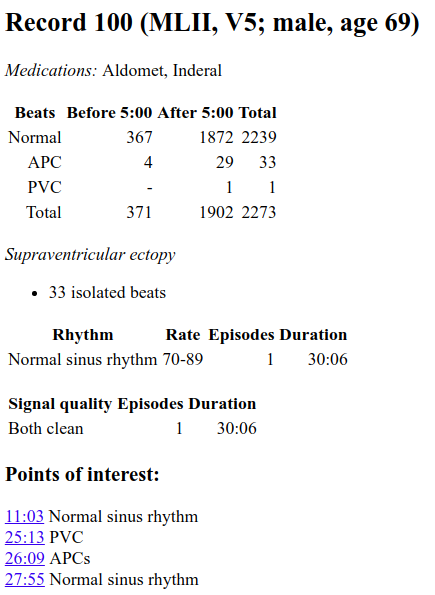
\includegraphics[scale=.6]{image/chapter2/record_info2.png}
    \begin{figure}[htp]
    \begin{center}
    \end{center}
    \caption{Thông tin bệnh nhân (bản ghi thứ 100)}
    \end{figure}
\end{center}
Mỗi bản ghi điện tim của bệnh nhân đều được ghi lại những thông tin về bệnh nhân đó. Những thông tin này không chỉ bao gồm những thông tin cơ bản trong quá trình ghi điện tầm đồ bình thường (Độ tuổi, giới tính, thuốc đang sử dụng điều trị,...) mà còn có những thông tin cần thiết cho quá trình nghiên cứu tim mạch (thống kê số nhịp bình thường và số nhịp bất thường, tần số từng loại nhịp, thời gian xuất hiện những nhịp đó,...)


\section{Mô hình để xuất}
Mô hình đề xuất trong nghiên cứu bao gồm 4 bước: trích xuất đặc trưng, xữ lý tín hiệu, phân chia tập dữ liệu, phân loại tín hiệu điện tâm đồ. Trong nghiên cứu này chúng tôi thực hiện 2 thí nghiệm, một thí nghiệm phân loại trên 1 đoạn RR để phát hiện loại nhịp và một thí nghiệm phân loại trên 20 đoạn RR liên tiếp.

\begin{center}
    
\includegraphics[scale=.5]{image/chapter5/system.png}
    \begin{figure}[htp]
    \begin{center}
    \end{center}
    \caption{Sơ đồ hệ thống phân loại điện tâm đồ}
    \end{figure}
\end{center}

\subsection{Trích xuất đặc trưng}
Giai đoạn trích xuất đặc trưng được xem là chìa khóa thành công trong việc phát hiện bất thường. Việc trích xuất đặc trưng của điện tim là việc cực kỳ quan trọn, đặc trưng được trích xuất ra phải bao hàm một lượng thông tin đáng kể để mô hình phân loại có thể dựa vào những thông tin đó đưa ra những quyết định chính xác. Trong hệ thống này, khoảng R-R (R-R interval) được trích xuất và được xem là đặc trưng của ECG. Theo Clifford và các cộng sự \cite{rr_clifford}, khoảng R-R chứa rất nhiều thông tin quan trọng của tim, đặc biệt là những thông tin về tình trạng bất thường ở tim. Chính vì thế nhiều nghiên cứu trong việc phân loại tín hiệu điện tâm đồ , phát hiện bất thường ở tim mạch sử dụng thông tin khoảng R-R. Ling và Yang \cite{Lin2013} đã chỉ ra rằng việc sử dụng khoảng R-R chuẩn hóa cải thiện đáng kể kết quả việc phân loại tín hiệu điện tâm đồ.

Dữ liệu sau khi xử lý tiền dữ liệu sẽ được trích xuất đặc trưng bằng kỹ thuật ngưỡng thích ứng kết hợp được đề xuất bới Christov. Những điểm R trong dữ liệu sẽ được đánh nhãn R.
\begin{center}
    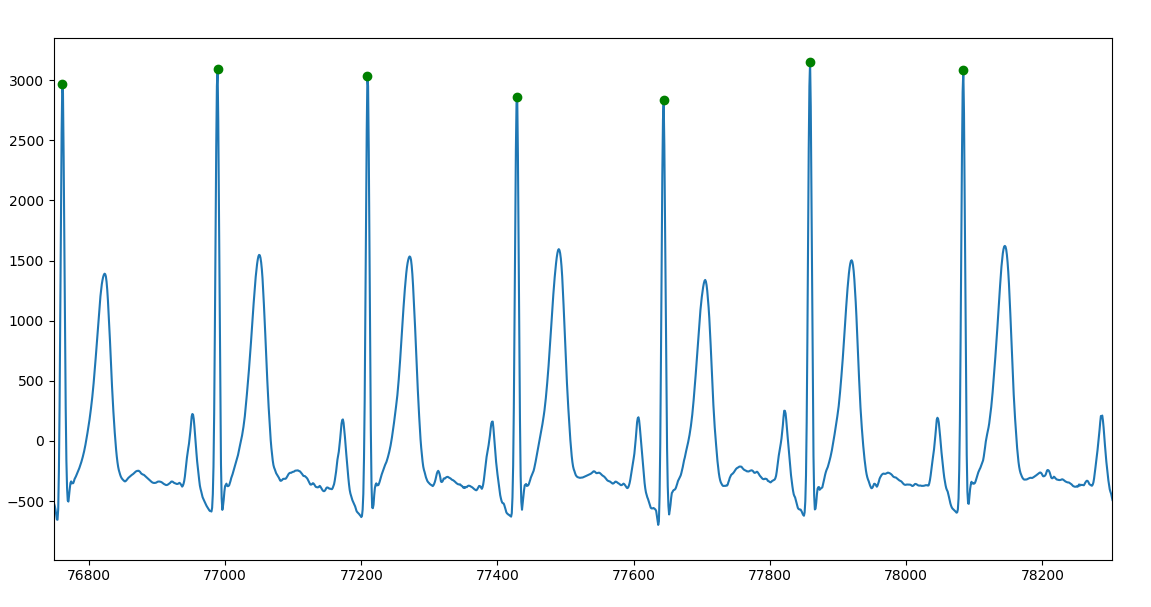
\includegraphics[scale=.3]{image/chapter5/R_detect.png}
    \begin{figure}[htp]
    \begin{center}
    \end{center}
    \caption{Hình ảnh đỉnh R được đánh dấu}
    \end{figure}
\end{center}

\subsection{Chuẩn hóa đặc trưng độ dài khoảng R-R}
Một trong những bước đặc biệt và có ảnh hưởng rất lớn đến chất lượng phân loại tín hiệu điện tâm đồ trong nghiên cứu này là việc chuẩn hóa hình dạng (shape normalization) cho đặc trưng khoảng R-R. Do đặc điểm sinh lý của tim mà các khoảng R-R thường có độ dài khác nhau (nhịp đập của tim thường không bất biến mà sẽ có một sự chênh lệch nhất định). Ở người bình thường, không mắc các bệnh lý về tim mạch, khoảng R-R sẽ dao động trong khoảng 600 – 1200 ms \cite{64} . Nếu sự không đồng nhất về mặt hình dạng của các khoảng R-R này không được giải quyết hiệu quả thì việc phân loại những tín hiệu điện tâm đồ mới, không có trong tập dữ liệu huấn luyện, sẽ gặp khó khăn và có thể dẫn đến kết quả phân loại, chẩn đoán không còn chính xác (trường hợp này được gọi là overfit – mô hình phân loại chỉ đáp ứng tốt với dữ liệu huấn luyện mà không còn đáp ứng tốt với dữ liệu kiểm thử hoàn toàn mới). Đó là lý do vì sao các khoảng R-R cần phải được chuẩn hóa về một hình dạng nhất định. Massagram và nhóm nghiên cứu \cite{67}, Bhola và nhóm nghiên cứu đều cho rằng 880 – 900 ms là khoảng thời gian phổ biến nhất của khoảng R-R \cite{68}.

Do đó, toàn bộ khoảng R-R trong nghiên cứu này sẽ được chuẩn hóa về khoảng thời gian đồng nhất 900 ms bằng phương pháp nội suy tuyến tính (linear interpolation). Hình dạng của khoảng R-R sau khi đã được chuẩn hóa đồng nhất về cùng một khoảng nhất định sẽ gần như không sai lệch quá nhiều so với khoảng R-R ban đầu.

\subsection{Xử lý tín hiệu}
Tín hiệu điện tâm đồ khi được thu nhận từ các thiết bị đo ban đầu có khả năng rất cao bị nhiễu do nhiều yếu tố khác nhau, như nhiễu do ảnh hưởng từ cơ bắp, nhiễu sinh ra từ các thiết bị điện tử, nhiễu từ các điện cực của thiết bị đo điện tâm đồ, power line interference, baseline wander,… Nhiễu có tác động rất lớn đến chất lượng của việc trích xuất đặc trưng và do đó ảnh hưởng đến kết quả bài toán phân loại (việc trích xuất đặc trưng từ tín hiệu điện tâm đồ có thể không chính xác và do đó có thể dẫn đến kết quả phân loại, chẩn đoán bị sai). Vì vậy, tín hiệu điện tâm đồ được thu nhận lúc ban đầu cần phải được khử nhiễu trước khi được đưa vào phân loại. Công đoạn khử nhiễu chúng tôi sử dụng kỹ thuật Phân tích thành phần chính (Principal component analys-PCA).
\begin{center}
        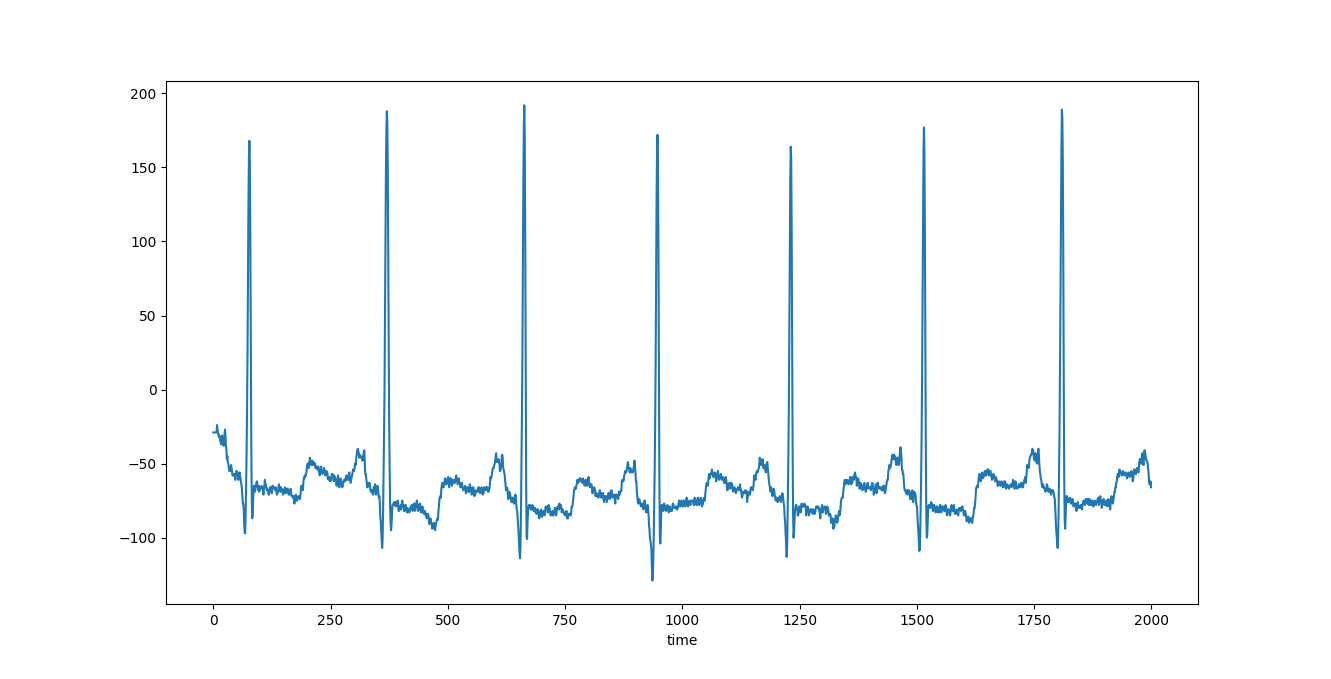
\includegraphics[width=.9\linewidth]{image/chapter5/noise.png}
        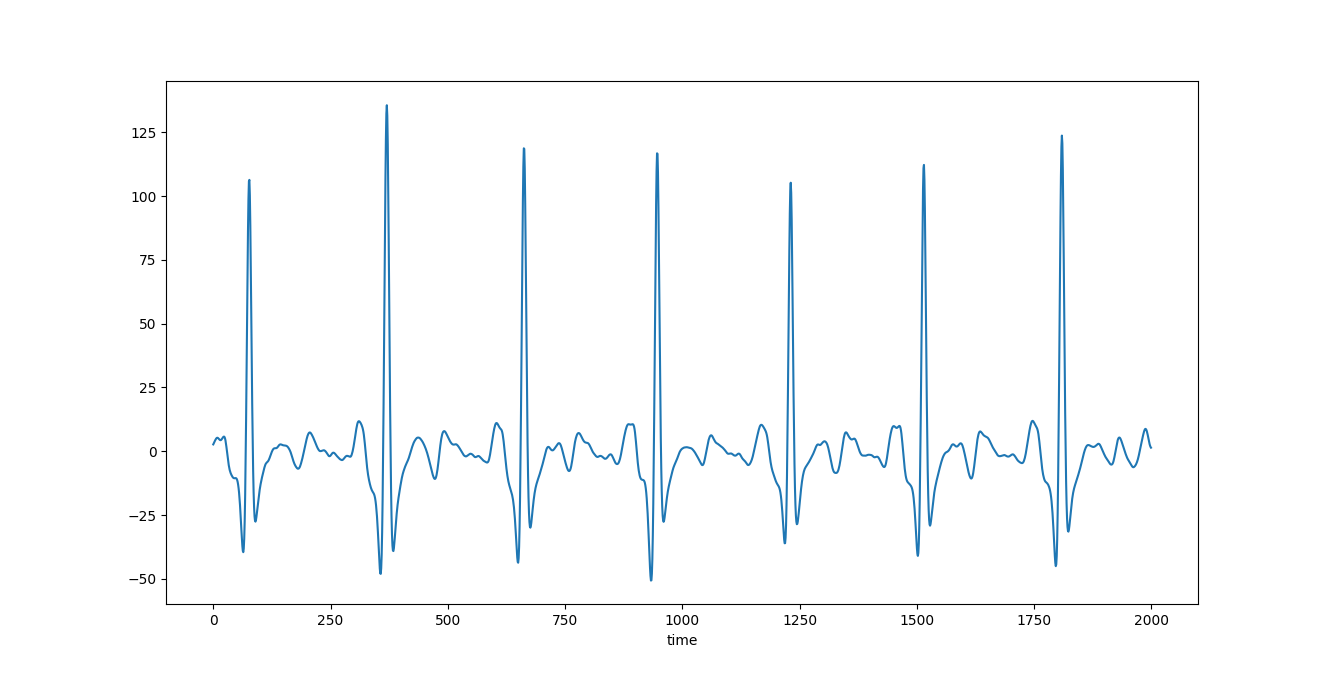
\includegraphics[width=.9\linewidth]{image/chapter5/hlp.png}
    \begin{figure}[!htb]
       \caption{Dữ liệu trước và sau khi lọc nhiễu}
    \end{figure}
\end{center}

\subsection{Phân chia tập dữ liệu}
Sau khi qua công đoạn trích xuất đặc trưng và khử nhiễu tiếp đến dữ liệu sẽ được xử lý để thực hiện thí nghiệm theo 2 hướng: 1 đoạn RR và 20 đoạn RR liên tiếp.
\subsubsection{Phân loại trên 1 đoạn RR}
Mỗi đoạn RR kể cả bất thường hay bình thường đều mang hình dáng đặc trưng, do hình dạng của điện tim mỗi người khác nhau phụ thuộc vào độ tuổi, giới tính và những đặc điểm khác. Một người có thể có hình dạng điện tâm đồ khác thường do tuổi tác và sử dụng thuốc điều trị mặc dù tim hoạt động bình thường. Dữ liệu đã đánh đỉnh R sẽ được cắt ra theo từng đoạn RR và xem như một dãy tín hiệu để đưa vào mô hình phân loại.

\subsubsection{Phân loại trên 20 đoạn RR liên tiếp}
Trong nghiên cứu cũng như chuẩn đoán y học, việc chuẩn đoán bệnh phải dựa trên một chuổi điện tim để quan sát hình dạng, sự thay đổi của điện tim về tần số, độ dài, biên độ. Mỗi mẫu điện tâm đồ dài vài chục giây thậm chí vài phút mà xuất hiện một đến một vài tín hiệu bất thường cũng được xem là bất thường. Mỗi đoạn RR sau khi xử lý sẽ được xem là một bước thời gian (timestep). Dữ liệu sẽ được cắt ra thành 20 đoạn RR liên tiếp bằng cách áp dụng kỹ thuật cửa sổ trược (sliding window) để tạo ra nhiều dữ liệu cho quá trình nghiên cứu. Mỗi 20 đoạn RR sẽ được đánh nhãn dựa trên nhãn của mổi đoạn RR chứa trong đó. Nếu trong đó có chứa 2 đoạn RR có nhãn bất thường trở lên (vì 2 đoạn RR sẽ chứa đầy đủ 6 tính chất sóng cơ bản nhất thể hiện bất thường) mẫu dữ liệu đó sẽ có nhãn bất thường.

\subsection{Mô hình phân loại}
\begin{center}
    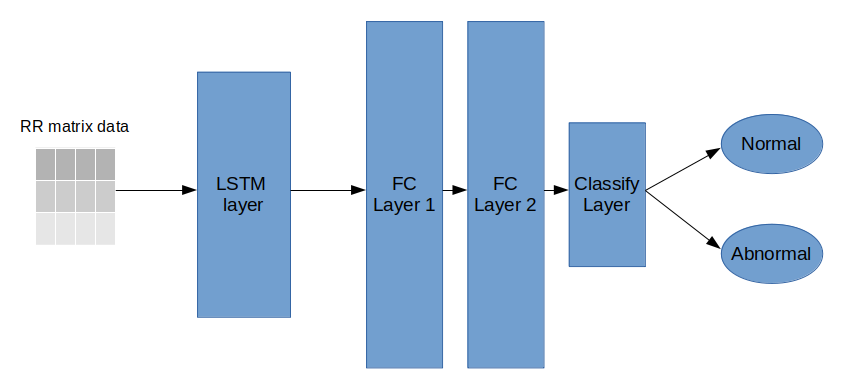
\includegraphics[scale=.4]{image/chapter5/model_architechture.png}
    \begin{figure}[htp]
    \begin{center}
    \end{center}
    \caption{Kiến trúc mô hình phân loại}
    \end{figure}
\end{center}
Mô hình phân loại tín hiệu điện tâm đồ gồm sự kết hợp giữa mạng LSTM và tầng Fully-connected. Trong đó:
\subsubsection{Mạng LSTM}
Mạng LSTM ở phần đầu của mô hình có chức năng học những đặc trưng tín hiệu điện tâm đồ có dạng Sequence-to-Sequence (Seq2Seq). Mạng LSTM sẽ học hình dáng của điện tâm đồ theo từng thí nghiệm để tiến hành phân loại qua bước tiếp theo. Số bước lặp mạng trong thí nghiệm 1 là 327 và thí nghiệm 2 là 20.
\subsubsection{Tầng Fully Connected}
Tầng Fully-connected có chức năng phân loại phân loại đã được học thành 2 nhãn Bình thường (0) và Bất thường (1).
Các tham số của mô hình phân loại:

\textbf{Tham số tốc độ học (learning rate)}: là 0.001 trên nguyên tắc thử sai nhiều lần, giá trị này ảnh hưởng đến tốc độ hội tụ của quá trình huấn luyện. (tốc độ học là một siêu tham số  được sử dụng trong đào tạo mạng lưới thần kinh có giá trị dương nhỏ, thường nằm trong khoảng giữa 0,0 và 1,0)

\textbf{Tầng Fully-Connected}: bao gồm 2 layer với 20 neural ẩn mỗi layer.

\textbf{Hàm biến đổi softmax} được áp dụng để phân loại 2 nhãn được gán đối với mỗi dữ liệu.

\begin{equation}
    S(y_i) = \frac{e^{y_i}}{\sum_{j=1}^{j}e^{y_i}}   
\end{equation}

\textbf{Hàm lỗi Cross-entropy} được sử dụng để phân loại nhãn Bình thường và Bất thường.

\begin{equation}
    L(y,p) = -\sum_{C}^{i=1}y_i\ln(p_i)
\end{equation}

\textbf{Các kỹ thuật tránh overfit} được áp dụng trên 2 layer Fully-connected để tránh overfitting dẫn đến sự sai lệch trong việc kiểm thử dữ liệu.
\begin{itemize}
    \item Chính quy hóa L2 (Relularization L2)
    \item Dropout
    \item Early Stopping
    \item Khởi tạo trọng số kiểu Xavier.
\end{itemize}

\textbf{Phương pháp tối ưu hóa hàm lỗi}: bộ tối ưu Adam.

\textbf{Số lần tính toán (epoch): 100}
